\documentclass[14pt, aspectratio=169]{beamer}
\usepackage[utf8]{inputenc}
\usepackage{graphicx, float}					% for images.
\graphicspath{{images/}}						% images directory.
\usetheme{CambridgeUS}
\usepackage{hyperref}							% external link.				
\usepackage{xcolor}								% color around link.
\setbeamertemplate{navigation symbols}{}		% hides navigation buttom at buttom of slides.
%\setbeamertemplate{headline}{}					% hides navigation bar at top.
\setbeamercovered{transparent}					% reveals next item. e.g. \item<1->
\setbeamertemplate{footline}[frame number]{}    % Show only page number in the footer.


\begin{document}
	\author{Shyarnis Ghising}
	\title{Getting started with Apache Airflow}
	\date{Dec 12, 2023}
	\titlegraphic{
\includegraphics[width=2cm]{airflow.png}}
	\subject{COMP 482}

	\begin{frame}[plain]
		\maketitle
	\end{frame}
	
	\begin{frame}[fragile]{Contents}
		\begin{columns}
			\column{0.6 \textwidth}
			\tableofcontents
			
			\column{0.3 \textwidth}
			
\includegraphics[width=4cm]{airflow.png}
		\end{columns}
	\end{frame}

	\section{Introduction}
	\begin{frame}{Introduction}
		\begin{itemize}
			\item<1-> Apache Airflow is a \textbf{batch-oriented} workflow for building data pipelines.
			\item<2-> It enables engineers to easily build \textbf{scheduled data pipelines} using a flexible Python framework.
			\item<3-> It \textbf{orchestrates} the different components responsible for processing data in data pipelines\cite{harenslak2020}.
		\end{itemize}
	\end{frame}
 
	\section{Data Pipelines}
	\begin{frame}{Data Pipelines}
		\begin{itemize}
			\item It consists of \textbf{several tasks} that needed to be executed.
			\item Tasks need to be executed in a \textbf{specific order}.
			\hspace{2cm}
			\begin{figure}[H]
				\centering
				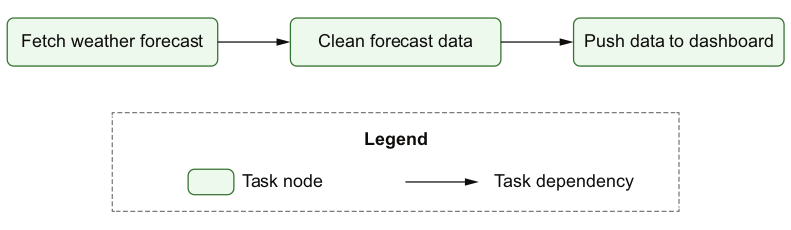
\includegraphics[width=13cm]{data-pipelines.png}
				\caption{Data Pipeline for the weather dashboard}
			\end{figure}
		\end{itemize}
	\end{frame}
	
	\subsection{Data pipelines as graphs}
	\begin{frame}{Data pipelines as graphs}
		\begin{itemize}
			\item \textbf{Tasks} are represented by  nodes/ vertices.
			\item \textbf{Dependenices between tasks} are represented by directed edges.
		\end{itemize}
		\begin{figure}[H]
			\centering
			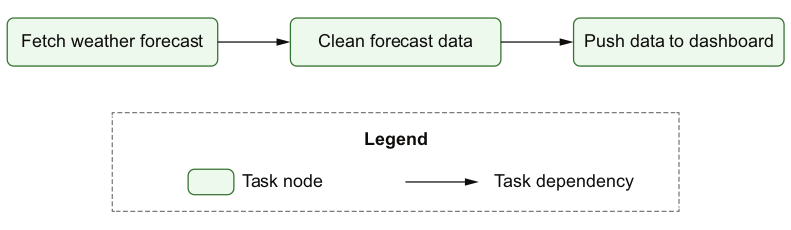
\includegraphics[width=13cm]{data-pipelines.png}
			\caption{Data Pipeline represented as DAG}
		\end{figure}
	\end{frame}

	\begin{frame}
		\begin{itemize}
			\item Such graphs are called \textit{directed acyclic graph} \textbf{DAG}.
			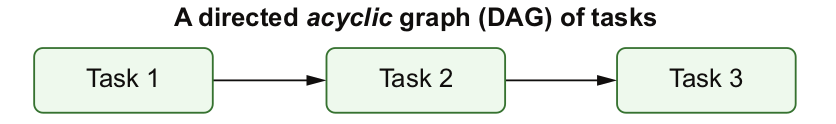
\includegraphics[width=9cm]{dag.png}
			
			\hspace{1cm}
			\item Directed cyclic graph leads to \textbf{deadlock} situation.
			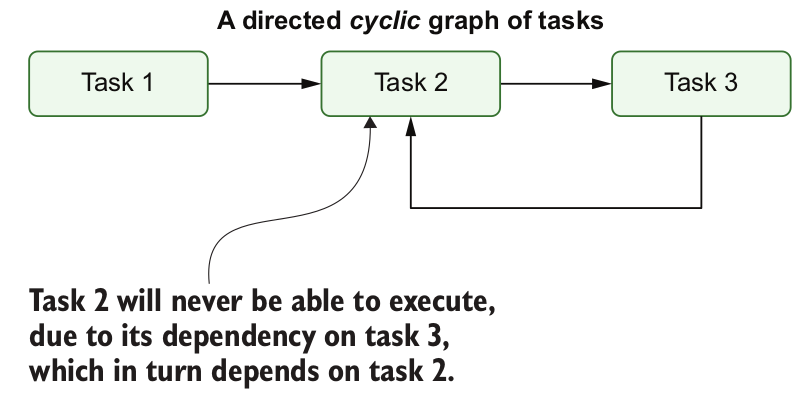
\includegraphics[width=8cm]{dcg.png}
		\end{itemize}
	\end{frame}

	\section{DAG in Python Code}
	\begin{frame}{DAG in Python Code}
		\begin{itemize}
			\item Python provide flexibility for building DAGs.
		\end{itemize}
		\begin{figure}[H]
			\centering
			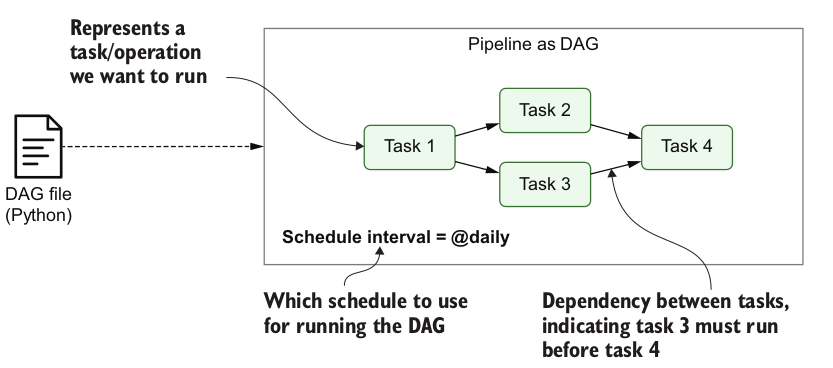
\includegraphics[width=10cm]{pipeline_as_dag.png}
			\caption{Pipelines are defined as DAGs using Python code}
		\end{figure}
	\end{frame}

	\section{Demonstration}
	\subsection{Installation}
	\begin{frame}{Installation}
		\href{https://airflow.apache.org/docs/apache-airflow/stable/start.html}{\fcolorbox{red}{white}{Install Airflow}} on your machine.		
		\begin{example}
			\texttt{
			- AIRFLOW\_VERSION==2.7.2\\
		    - PYTHON\_VERSION==3.8 \\
		    - pip install "apache-airflow==2.7.2" --constraint\\ 
			 "https://raw.githubusercontent.com/apache/airflow/ \\
			 constraints-2.7.2/constraints-no-providers-3.8.txt"
			}
		\end{example}
		\href{https://raw.githubusercontent.com/apache/airflow/constraints-2.7.3/constraints-3.8.txt}{\fcolorbox{red}{white}{constraints}}
	\end{frame}

	\begin{frame}
		\begin{itemize}
			\item airflow db migrate
			\item \texttt{airflow users create --username <usernname> --password <password> --firstname <fanme> --lastname <lname> --role Admin --email <email>}
			\item airflow scheduler
			\item airflow webserver
		\end{itemize}
	\end{frame}

	\begin{frame}
		\begin{figure}
			\centering
			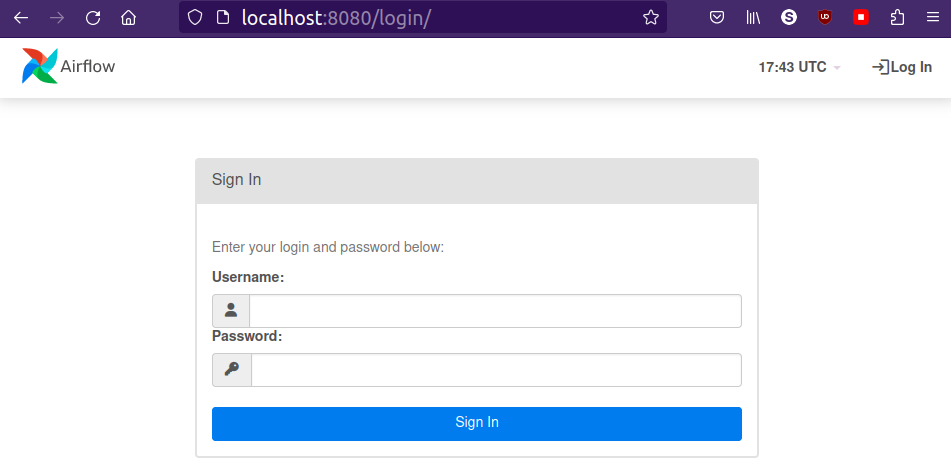
\includegraphics[width=14cm]{airflow-login.png}
			\caption{Airflow login view}
		\end{figure}
	\end{frame}
	
	\begin{frame}
		\begin{figure}
			\centering
			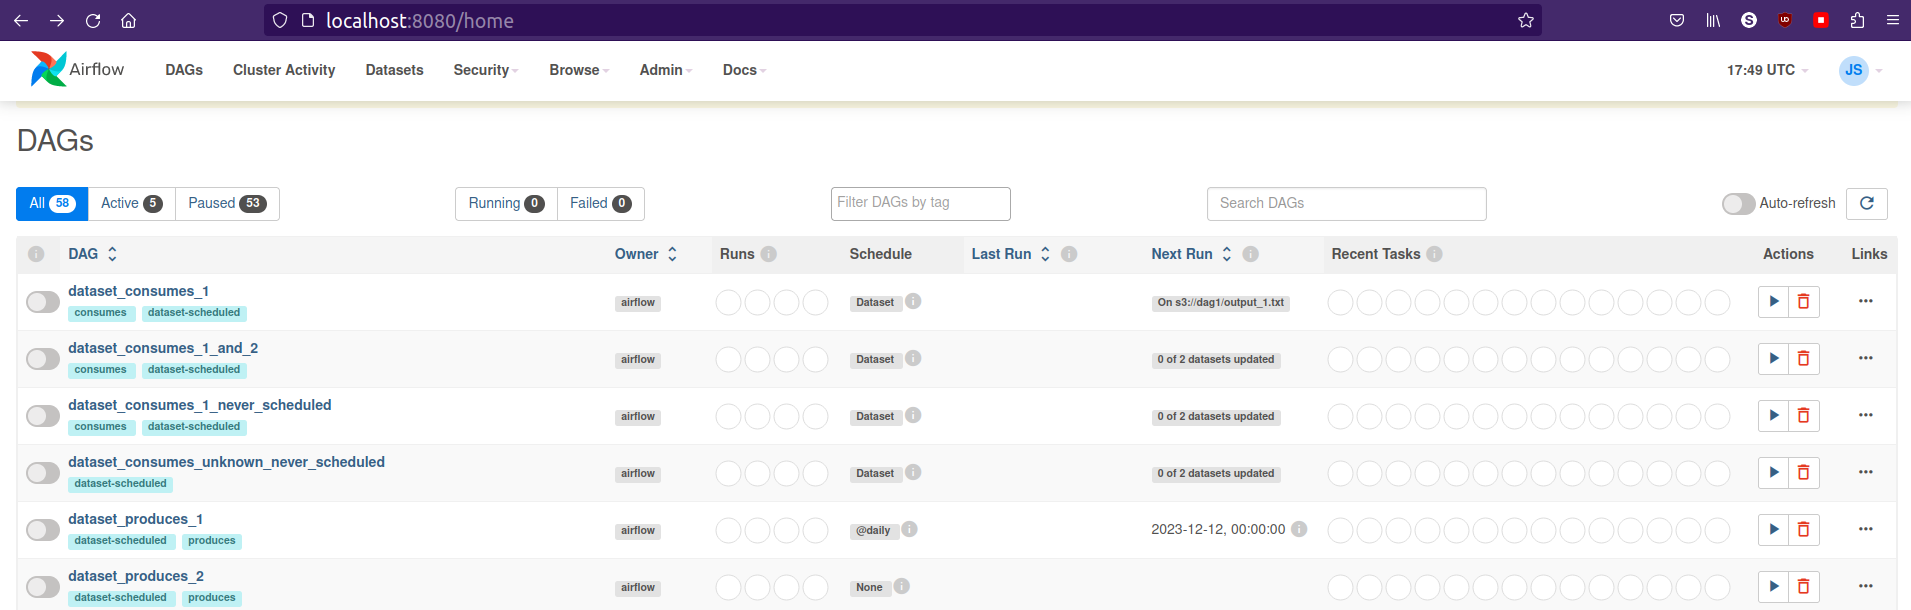
\includegraphics[width=15cm]{list-of-dags.png}
			\caption{List of Airflow DAG}
		\end{figure}
	\end{frame}

	\begin{frame}
		\begin{figure}
			\centering
			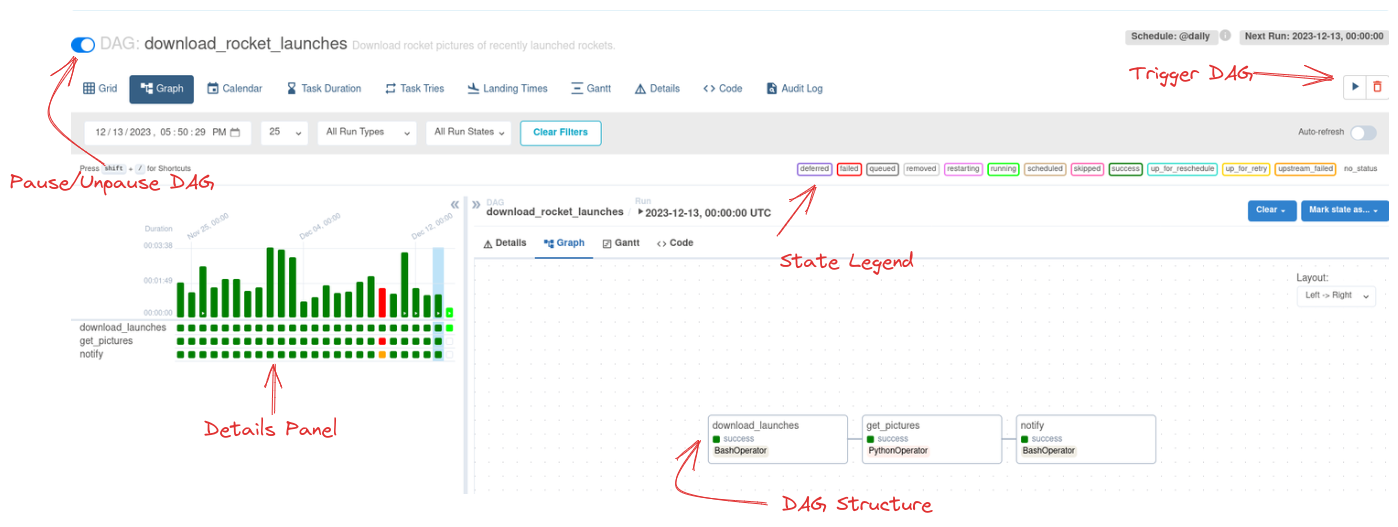
\includegraphics[width=15cm]{airflow-mapped.png}
			\caption{Airflow DAG in Action}
		\end{figure}
	\end{frame}

	\subsection{Live Demonstration}
	\begin{frame}{Live Demonstration}
		\begin{figure}[H]
			\centering
			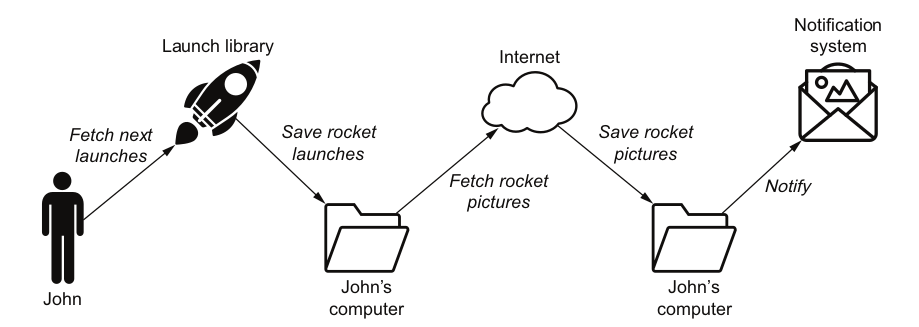
\includegraphics[width=12cm]{mental_model.png}
			\caption{John’s mental model of downloading rocket pictures}
		\end{figure}
	\end{frame}

	\begin{frame}
		\begin{figure}[H]
			\centering
			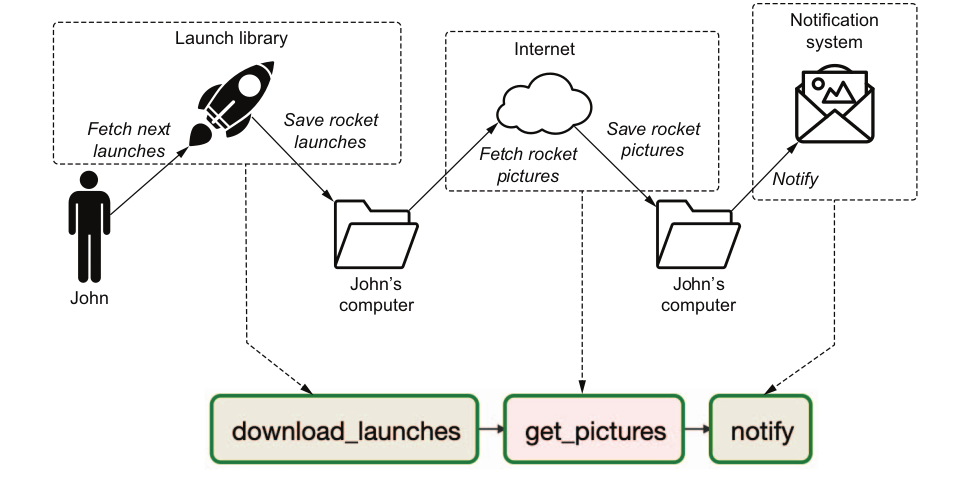
\includegraphics[width=12cm]{mapped.png}
			\caption{John’s mental model mapped to tasks in Airflow}
		\end{figure}
	\end{frame}

	\section{References}
	\begin{frame}{References}
		\bibliographystyle{unsrt}
		\bibliography{bibliography}
	\end{frame}

\end{document}